\begin{problem}
  A small Lambertian source $\d A$ is centered at $P$
  and emits radiance $L$. The orientation of this patch is the same
  as that of a plane containing two points, $X_1$ and $X_2$.
  The point $X_1$ is the point on this plane that is closest to $P$,
  and the distance from $P$ to $X_1$ is $D$ as shown.
  \begin{figure}[H]
    \centering
    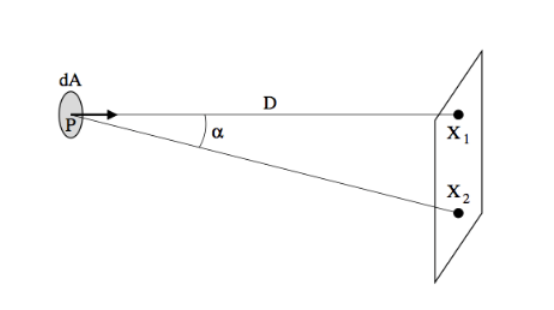
\includegraphics[width=0.5\textwidth]{figures/lambertian.png}
    \label{fig:1}
  \end{figure}
  \begin{enumroman}
    \item Calculate the solid angle subtended by $\d A$ at points $X_1$ and $X_2$.
      \begin{answer}
        
      \end{answer}
    \item Calculate the irradiance $E$ incident on the plane at points $X_1$ and $X_2$,
      and calculate the ratio $E(X_1)/E(X_2)$.
      \begin{answer}
        
      \end{answer}
  \end{enumroman}
\end{problem}

